\subsection*{Model}
The function described in this problem is the following
\begin{equation*}
    \begin{aligned}
    & F(\mathbf{x}) = \frac{1}{2} \sum_{k=1}^{n} f_k^2(x) \\
    & f_k(\mathbf{x}) = x_k - \frac{x_{k+1}^2}{10}, \quad   1 \leq k < n \\   
    & f_n(\mathbf{x}) = x_n - \frac{x_1^2}{10}
    \end{aligned}
\end{equation*}
where $n$ denotes the dimensionality of the input vector $\mathbf{x}$.
\\ The starting point for the minimization is the vector $\mathbf{x}_0 = [2, 2, \ldots, 2]$.


To be able to say something more about the behaviour of the problem is useful to look at the gradient of the function $F(\mathbf{x})$ and at its Hessian matrix.
\begin{equation*}
    \nabla F(\mathbf{x}) = 
    \begin{bmatrix}
        \frac{\partial F}{\partial x_1}(\mathbf{x}) \\
        \vdots \\
        \frac{\partial F}{\partial x_k}(\mathbf{x}) \\
        \vdots \\
        \frac{\partial F}{\partial x_n}(\mathbf{x})
    \end{bmatrix}
    =
    \begin{bmatrix}
        \frac{\partial}{\partial x_1} \frac{1}{2}\left[f_n^2 + f_1^2\right] (\mathbf{x})\\
        \vdots \\
        \frac{\partial}{\partial x_k} \frac{1}{2}\left[f_{k-1}^2 + f_k^2\right] (\mathbf{x})\\
        \vdots \\
        \frac{\partial}{\partial x_n}  \frac{1}{2}\left[f_{n-1}^2 + f_n^2\right] (\mathbf{x})
    \end{bmatrix}
    =
    \begin{bmatrix}
        -\frac{x_1}{5}\left(x_n - \frac{x_1^2}{10}\right) + \left(x_1 - \frac{x_1^2}{10}\right) \\
        \vdots \\
        -\frac{x_k}{5}\left(x_{k-1} - \frac{x_k^2}{10}\right) + \left(x_k - \frac{x_{k+1}^2}{10}\right) \\
        \vdots \\
        -\frac{x_n}{5}\left(x_{n-1} - \frac{x_n^2}{10}\right) + \left(x_n - \frac{x_1^2}{10}\right)
    \end{bmatrix}
\end{equation*}
Due to the particular structure of the function, the Hessian matrix as a sparse structure, with only 3 diagonals different from zero. The non-zero elements are the following:
\begin{align*}
    \frac{\partial^2 F}{\partial x_k^2} (\mathbf{x}) &= -\frac{1}{5}x_{k-1} - \frac{3}{50}x_k^2  + 1, \quad 1 < k \leq n  &
    \frac{\partial^2 F}{\partial x_1^2} (\mathbf{x}) &= -\frac{1}{5}x_{n} - \frac{3}{50}x_1^2  + 1, \\
    \frac{\partial^2 F}{\partial x_k \partial x_{k+1}} (\mathbf{x}) &= -\frac{1}{5}x_{k+1}, \quad 1 \leq k < n  &
    \frac{\partial^2 F}{\partial x_n \partial x_1}(\mathbf{x}) &= -\frac{1}{5}x_1  \\
    \frac{\partial^2 F}{\partial x_k \partial x_{k-1}}(\mathbf{x}) &= -\frac{1}{5}x_{k}, \quad 1 < k \leq n  &
    \frac{\partial^2 F}{\partial x_1 \partial x_{n}}(\mathbf{x}) &= -\frac{1}{5}x_{n}
\end{align*}
We can now easily notice that the gradient of the function is null when all the components of the vector $\mathbf{x}$ are equal to 0, in this case the Hessian matrix is positive definite, so the point $\mathbf{x} = \mathbf{0}$ is a minimum of the function $F(\mathbf{x})$. 
Because of the definition of the function, $0$ is the lowest value the function can assume, so the minimum found is global.


\medskip
\subsection*{Nealder Mead Method}
We now report a table containing some general results obtained by running the Nealder Mead method on the function $F(\mathbf{x})$.

\begin{figure*}[htbp]
    \centering
    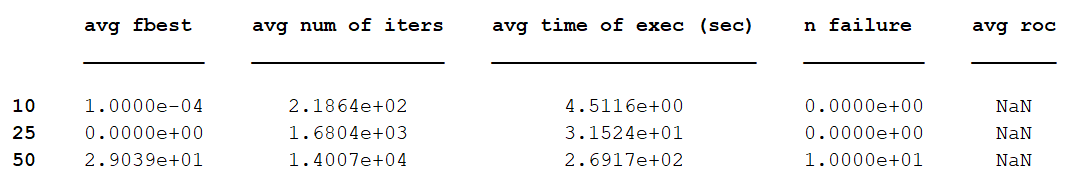
\includegraphics[width = 0.9\textwidth]{img/pb76_table_SX.png}
    \caption{Resultats obtained by running the symplex method on the problem $76$.}
\end{figure*}

First thing we can notice is that for smaller dimensionalities the symplex method is able to find the minimum in a reasonable amount of time, but when the dimensionality becomes higher the method starts failing.
From the plot in figure $\eqref{fig:iter}$, we can see that for most points belonging to $\mathbb{R}^{50}$, the method keeps iterating until the maximum number of iterations is reached without satisfying the stopping criterion.
This behaviour can probably be explained by the fact that when the dimensionality increases the starting point is more far from the minimum due to its definition, so the method needs to perform more iterations to reach the minimum.
\begin{figure}[htbp]
    \centering
    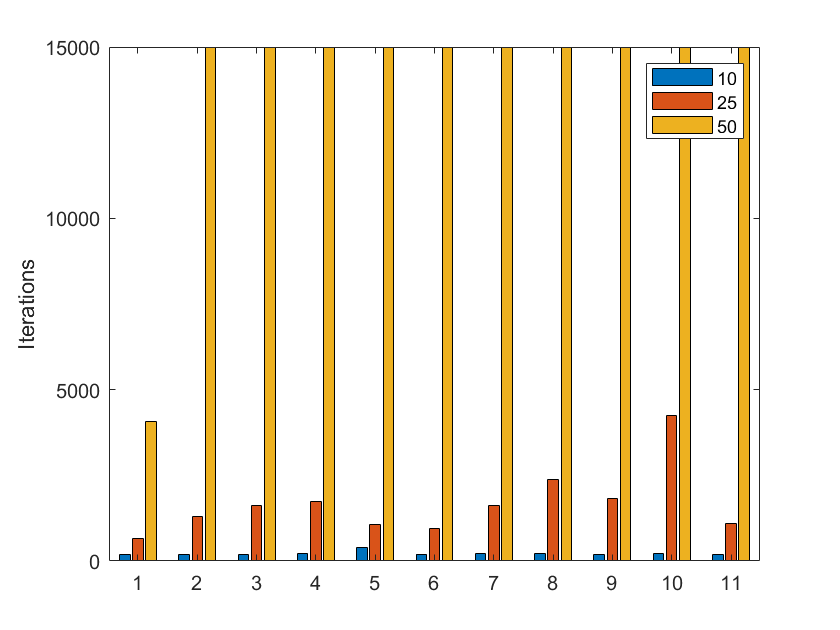
\includegraphics[width = 0.5\textwidth]{img/pb76_SX_iter.png}
    \caption{Number of iterations needed by the Nealder Mead method to find the minimum of the problem $76$ for each starting point.}
    \label{fig:iter}
\end{figure}

From the previous table, we can notice that the experimental rate of convergnce is always \verb+Nan+: this is due to the fact that in the last iterations the value of $\mathbf{x}^{(k)}$ does not change much and thus it yields a division by zero in the formula $\eqref{definizione_roc}$ which defines the experimental rate of convergence.
This can be seen in the following plots, showing that, in the last iterations, the approximated value of the minimum seems to be stationary.
\begin{figure}[htbp]
    \centering
    % Prima immagine
    \begin{subfigure}[t]{0.35\textwidth}  % Larghezza del 45% del testo
        \centering
        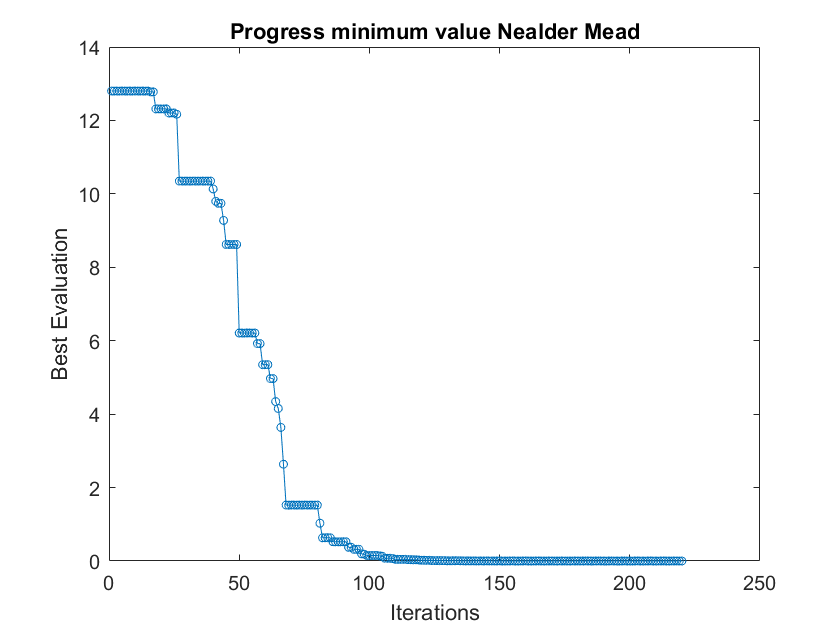
\includegraphics[width=\textwidth]{img/pb76_SX_es10.png}
        \caption{dimension $10$}
        \label{fig:R6}
    \end{subfigure}
    \hspace{1cm} %spaziatura tra le immagini
    % Seconda immagine
    \begin{subfigure}[t]{0.35\textwidth}
        \centering
        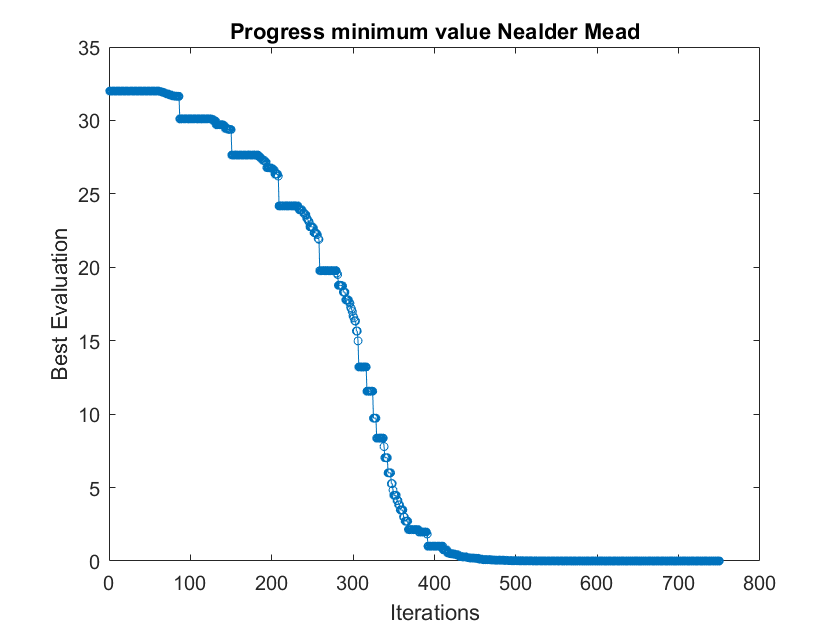
\includegraphics[width=\textwidth]{img/pb76_SX_es25.png}
        \caption{dimension $25$}
        \label{fig:R8}
    \end{subfigure}
    % Didascalia generale
    \caption{ \small Plots of the progresses of the Nealder Mead method for different dimensionalities for the problem $76$.}
    \label{fig:overall}
\end{figure}


\medskip
\subsection*{Modified Newton Method - Exact Derivatives}
We now report a table containing some general results obtained by running the Modified Newton method on the function $F(\mathbf{x})$.
We obviously expect the method to perform better than the symplex method because of the exact derivatives used in the computation of the descent direction.

\begin{figure*}[htbp]
    \centering
    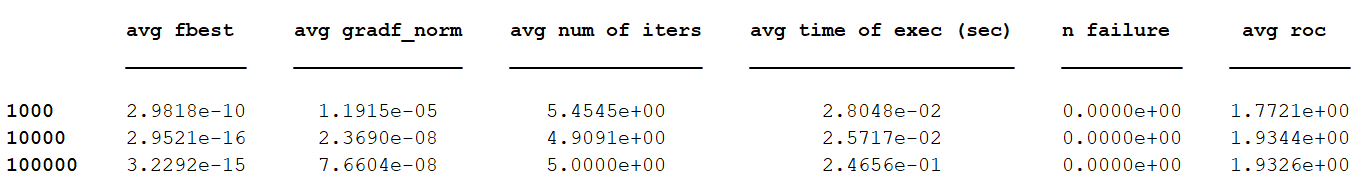
\includegraphics[width = 0.9\textwidth]{img/pb76_table_MN.png}
    \caption{Resultats obtained by running the Modified Newton Method on the problem $76$ using the exact derivatives.}
\end{figure*}

This time, the method always converges to the minimum point in very few iterations, even for higher dimensionalities. 
We can also appreciate the fact that the approximated rate of convergence is close to $2$, as expected for a Newton method.
Comparing this table with the previous one (showing the results obtained by running the symplex method), we can see that the Modified Newton method identifies as minimum a point in which the evaluation of the function is much smaller. 
This behavior aligns with theoretical expectations, as the Modified Newton method leverages the exact derivatives of the function $F(\mathbf{x})$ to determine the descent direction, while the symplex method depends only on function evaluations.

\medskip
\subsection*{Modified Newton Method - Approximated Derivatives}
Approximating the derivatives of the function $F(\mathbf{x})$ using finite differences is more challenging than it appears due to potential numerical cancellation issues, which can occur when subtracting two nearly equal quantities. Additionally, we aim to derive a formula that minimizes computational cost.

Let's begin by approximating the first-order derivatives of the function $F(\mathbf{x})$ using the centered finite difference formula with step $h_k$. The subscript $k$ is specified because the following formula are valid both with a constant increment, $h_k = k$ for all $h = 1, \dots, n$, and with a specific increment $h_k = h |\hat{x}_k| \; k= 1, \dots, n$, where $\mathbf{\hat{x}}$ is the point at which we approximate the derivatives.
$$ \frac{\partial F }{\partial x_k} (\mathbf{x}) \approx \frac{F(\mathbf{x} + h_k \vec{e}_k) - F(\mathbf{x} - h_k \vec{e}_k)}{2h_k} = 
\frac{\sum_{i = 1}^{n} f_i(\mathbf{x} + h_k \vec{e}_k)^2 - \sum_{i = 1}^{n} f_i(\mathbf{x} - h_k \vec{e}_k)^2}{4h_k}$$
We can observe that each term $f_i^2$ only depends on $x_i$ and $x_{i+1}$, so $f_i(\mathbf{x} + h_k\vec{e}_k)^2 - f_i(\mathbf{x} - h_k\vec{e}_k)^2 = 0$ for all $i \neq k-1, k$ (or $i \neq 1,n$ if we are considering $k = 1$). 
This allows to simplify the formula, even in order to decrease the computational cost, as follows
$$\frac{\partial F }{\partial x_k} (\mathbf{x}) \approx  \frac{f_{k-1}(\mathbf{x} + h_k\vec{e}_k)^2 - f_{k-1}(\mathbf{x} - h_k\vec{e}_k)^2 + f_{k}(\mathbf{x} + h_k\vec{e}_k)^2 - f_{k}(\mathbf{x} - h_k\vec{e}_k)^2}{4h_k}  \quad 1 < k \leq n$$
$$\frac{\partial F }{\partial x_k} (\mathbf{x}) \approx  \frac{f_{n}(\mathbf{x} + h_k\vec{e}_k)^2 - f_{n}(\mathbf{x} - h_k\vec{e}_k)^2 + f_{k}(\mathbf{x} + h_k\vec{e}_k)^2 - f_{k}(\mathbf{x} - h_k\vec{e}_k)^2}{4h_k}  \quad k = 1$$
In order to avoid numerical cancellation, the numerator has been expanded obtaining the following formula
\begin{align*}
    \frac{\partial F }{\partial x_1} (\mathbf{x}) & \approx \frac{4h_k x_1 - 2/5 h_k x_2^2 - 4/5 h_k x_n x_1 + 8/100 h_k x_1 (x_1^2 + h_k^2)}{4h_k} \\
    \frac{\partial F }{\partial x_k} (\mathbf{x}) & \approx \frac{4h_k x_k - 2/5 h_k x_{k+1}^2 - 4/5 h_k x_{k-1} x_k + 8/100 h_k x_k (x_k^2 + h_k^2)}{4h_k} \\
    \frac{\partial F }{\partial x_n} (\mathbf{x}) & \approx \frac{4h_k x_n - 2/5 h_k x_{1}^2 - 4/5 h_k x_{n-1} x_n + 8/100 h_k x_n (x_n^2 + h_k^2)}{4h_k}
\end{align*}


We can now proceed to approximate the second order derivatives of the function $F(\mathbf{x})$ using the centered finite difference formula; this time we need to use two different increments $h_i$ and $h_j$ based on the two components with respect to which we are differentiating.
The general formula is the following
$$ \frac{\partial^2 F}{\partial x_i \partial x_j} (\mathbf{x})  = \frac{F(\mathbf{x} + h_i \vec{e}_i + h_j \vec{e}_j) - F(\mathbf{x} + h_i \vec{e}_i) - F(\mathbf{x} - h_j \vec{e}_j) + F(\mathbf{x})}{h_i h_j}$$

The approximation of the Hessian matrix has to be approached taking into account its sparsity in order to reduce the computational cost, indeed in the Matlab script we have implemented a function that approximates the Hessian matrix just by computing the non-null terms which are the following
\begin{align*}
    & \frac{\partial^2 F}{\partial x_k^2} (\mathbf{x})  \approx 2h_k - \frac{2}{5} x_{k-1} h_k + \frac{12}{100} x_k^2 h_k^2 + \frac{24}{100}x_k h_k^3 + \frac{14}{100} h_k^2 \quad & 1 < k \leq n \\
    & \frac{\partial^2 F}{\partial x_k^2} (\mathbf{x})  \approx 2h_k - \frac{2}{5} x_{n} h_k + \frac{12}{100} x_k^2 h_k^2 + \frac{24}{100}x_k h_k^3 + \frac{14}{100} h_k^2 \quad  & k = 1 \\
    & \frac{\partial^2 F}{\partial x_k \partial x_{k+1}} (\mathbf{x})  \approx - \frac{2}{5} h_k h_{k+1} x_{k+1} - \frac{1}{5} h_k^2 h_{k+1} \quad & 1 \leq k < n 
\end{align*}
The values of the inferior diagonal are obtained by exploiting the symmetry of the Hessian matrix.

The terms have been computed following the same approach described above: the numerator has been expanded negletting the $f_i^2()$ that are not affected by the varation of the components with respect to which we are differentiating.


We now report some barplots showing the results obtained by running the Modified Newton method on the function $F(\mathbf{x})$ using the approximated derivatives.

\begin{figure}[htbp]
    \centering
    % Prima immagine
    \begin{subfigure}[t]{0.45\textwidth}  % Larghezza del 45% del testo
        \centering
        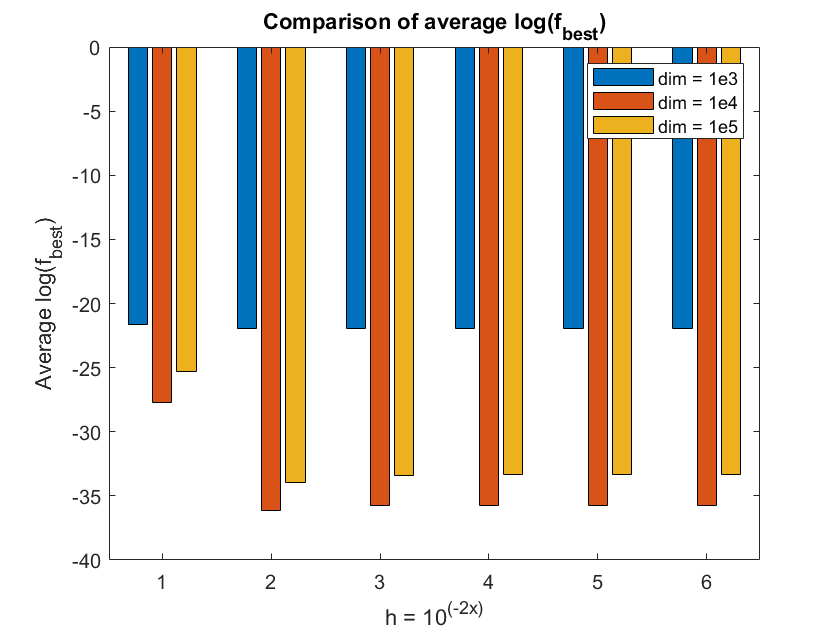
\includegraphics[width=\textwidth]{img/pb76_MN_difffinite_COST_log(fbest).png}
        \caption{Costant Increment $h$}
    \end{subfigure}
    \hspace{1cm} %spaziatura tra le immagini
    % Seconda immagine
    \begin{subfigure}[t]{0.45\textwidth}
        \centering
        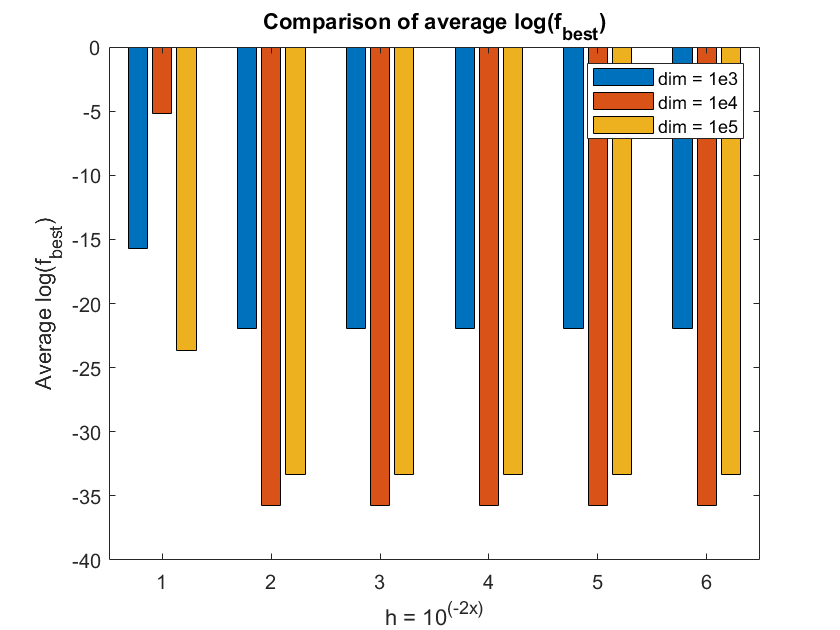
\includegraphics[width=\textwidth]{img/pb76_MN_difffinite_REL_log(fbest).png}
        \caption{Specific Increment }
    \end{subfigure}
    % Didascalia generale
    \caption{ \small Values of the average $\log(f_{best})$ in function of the increment while running the Modified Newton Method with approximated derivatives on the problem $76$.}
    \label{logfbest_difffinite}
\end{figure}

As we can see from the plots $\eqref{logfbest_difffinite}$, expecially for larger values of the increments, the algorithm converges to a point such that the value of the function is higher accordingly to the fact that the approximated derivatives are less accurate. Nonetheless, the method succeeds to find an acceptable approximation of the minimum value even when computing the descent direction with just an approximation of the derivatives.

\begin{figure*}[htbp]
    \centering
    % Prima immagine
    \begin{subfigure}[t]{0.45\textwidth}  % Larghezza del 45% del testo
        \centering
        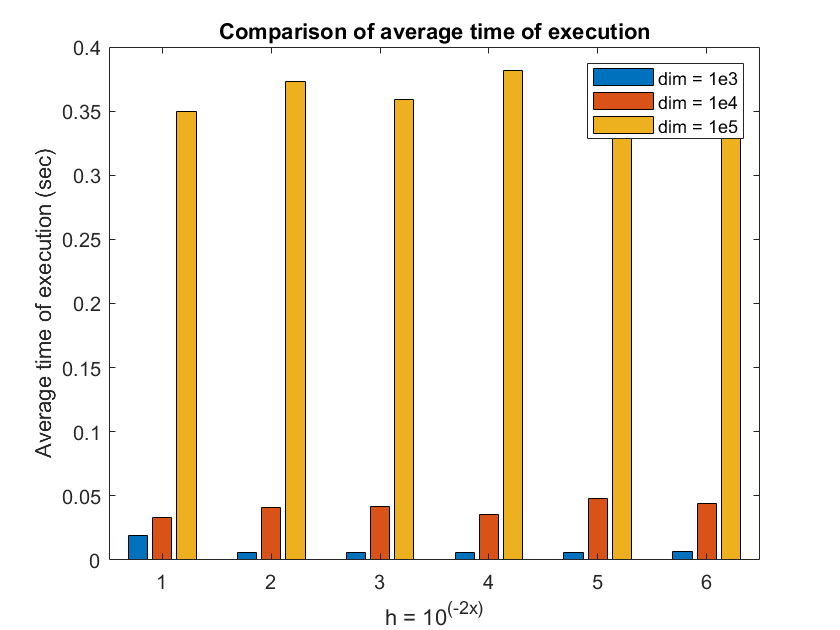
\includegraphics[width=\textwidth]{img/pb76_MN_difffinite_COST_timeofexec.png}
        \caption{Costant Increment $h$}
    \end{subfigure}
    \hspace{1cm} %spaziatura tra le immagini
    % Seconda immagine
    \begin{subfigure}[t]{0.45\textwidth}
        \centering
        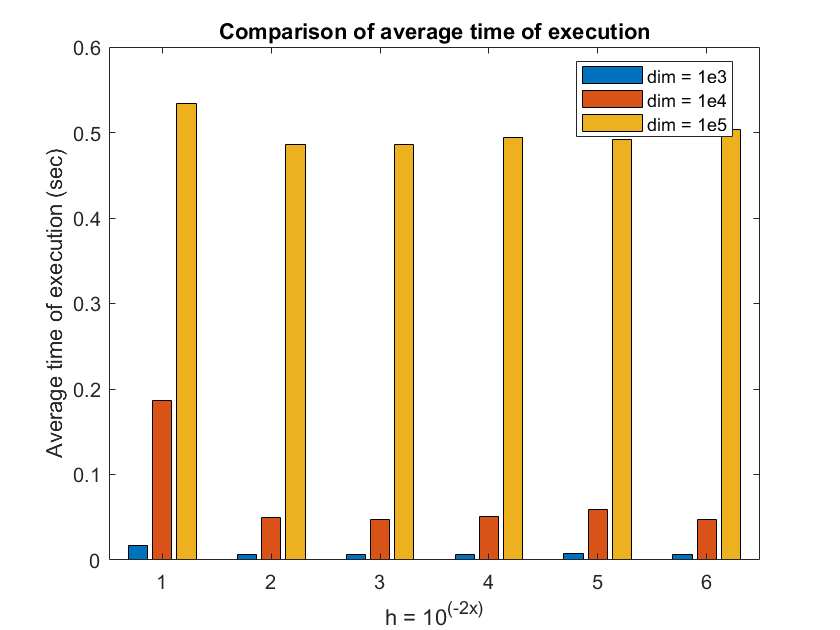
\includegraphics[width=\textwidth]{img/pb76_MN_difffinite_REL_timeofexec.png}
        \caption{Specific Increment }
    \end{subfigure}
    % Didascalia generale
    \caption{ \small Average time of execution in function of the increment $h$  while running the Modified Newton Method with approximated derivatives on the problem $76$.}
\end{figure*}


\begin{figure*}[htbp]
    \centering
    % Prima immagine
    \begin{subfigure}[t]{0.45\textwidth}  % Larghezza del 45% del testo
        \centering
        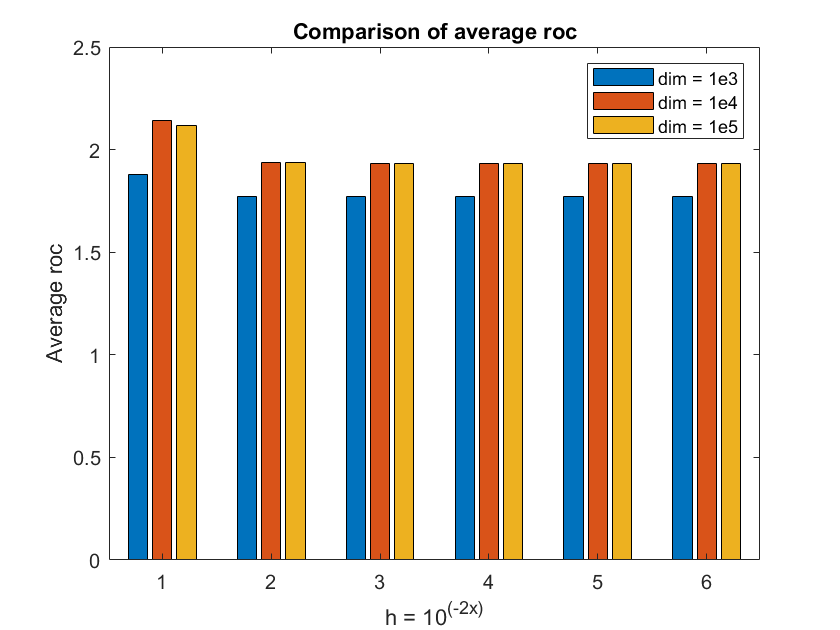
\includegraphics[width=\textwidth]{img/pb76_MN_difffinite_COST_rateofconv.png}
        \caption{Costant Increment $h$}
    \end{subfigure}
    \hspace{1cm} %spaziatura tra le immagini
    % Seconda immagine
    \begin{subfigure}[t]{0.45\textwidth}
        \centering
        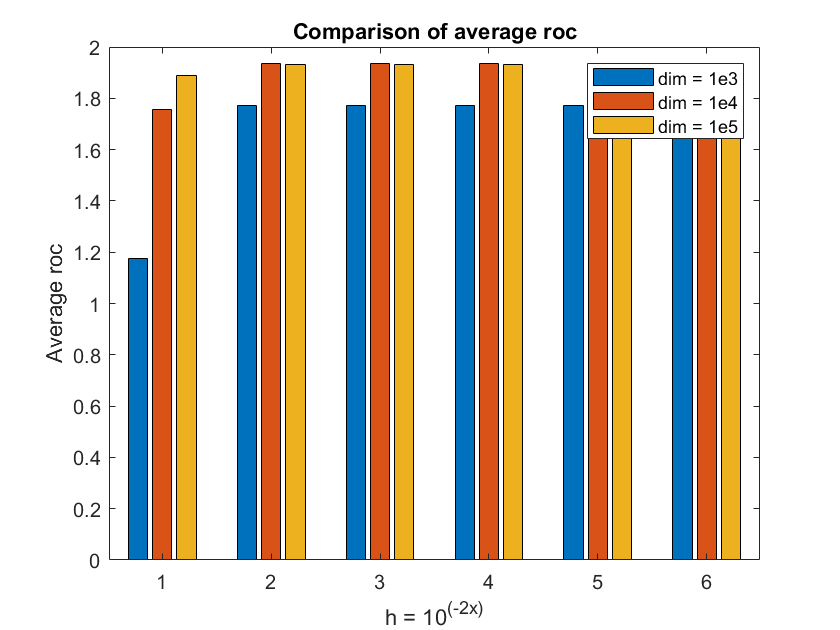
\includegraphics[width=\textwidth]{img/pb76_MN_difffinite_REL_rateofconv.png}
        \caption{Specific Increment }
    \end{subfigure}
    % Didascalia generale
    \caption{ \small Average values of the experimental rate of convergence in function of the increment $h$  while running the Modified Newton Method with approximated derivatives on the problem $76$.}
\end{figure*}


The others plots show that the average time of execution and the average rate of convergence are not significantly affected by the approximation of the derivatives for none of the values oh the increment $h$.